%%%%%%%%%%%%%%%%%%%%%%%%%%%%%%%%%%%%%%%%%%%%%%%%%%%%%%%%%%%%%%%%%%%%%%%%%%%%%%%%


%\documentclass[letterpaper, 10pt, conference]{IEEEtran}
\documentclass[notes]{beamer}
\usepackage{tikz}
\usetikzlibrary{calc,decorations.markings,arrows, fadings}
\usepackage{tikz-timing}
\usepackage{amsmath}
\usepackage{xifthen}
\usepackage{amsfonts}
\usepackage{tabu}
\usepackage{graphicx,dblfloatfix}
\usepackage[font=small]{caption}
%\usepackage{subcaption}
\usepackage{cite}
\usepackage{placeins}
\usepackage{xspace}
\usepackage{subfiles}
\usepackage{url}
\usepackage[outline]{contour}

\contourlength{0.18em}

\usetheme{Copenhagen}
\usecolortheme{beetle} 
%\setbeamertemplate{navigation symbols}{}
\beamertemplatenavigationsymbolsempty
\setbeamerfont{footline}{series=\scriptsize}
\usefonttheme{structurebold}

\definecolor{beetle@other}{RGB}{207,184,124} %cu gold
%
%Once I break this in to multiple sections, each section will be added with:
%	\subfile{filename}
%In those other files, I have as preamble:
%	\documentclass[main.tex]{subfiles}
%

\title[\textcolor{black}{Low-Cost Omnidirectional Powertrain}]{A Stick-Slip Omnidirectional Powertrain for Low-Cost Swarm Robotics:\\ Mechanism, Calibration, and Control}
\author[{\tt john.klingner@colorado.edu}]{John Klingner, Anshul Kanakia, Nicholas Farrow, Dustin Reishus and Nikolaus Correll}
\institute[]{Department of Computer Science\\University of Colorado Boulder}
\date{}

\newcommand{\Tau}{\boldsymbol{\mathrm{T}}}

\begin{document}
\begin{frame}
	\titlepage
\end{frame}
\begin{frame}{Motivation \& Background}
\begin{columns}[c]
	\column{0.65\textwidth}
		\begin{itemize}
			\item Stick-slip motion.
				\note[item]<1->{
					\begin{itemize}
						\item Primary goal is to effect motion cheaply.
						\item Uses the impulse forces generated by vibration motors (cost: $\frac{\$0.50}{\text{unit}}$) to "scoot" the robot along.
					\end{itemize}
				}
			\item Previous work.
				\note[item]<1->{
					\begin{itemize}
						\item Has demonstrated the efficacy of this approach for skid steering motion driven by two motors. This work determined that a three-motor setup with holonomic drive was infeasible in real robots. [Vartholomeos 2006]
						\item We extend this work to allow for an omnidirectional powertrain using three motors.
					\end{itemize}
				}
		\end{itemize}
	\column{0.35\textwidth}
		\begin{figure}
			\centering
			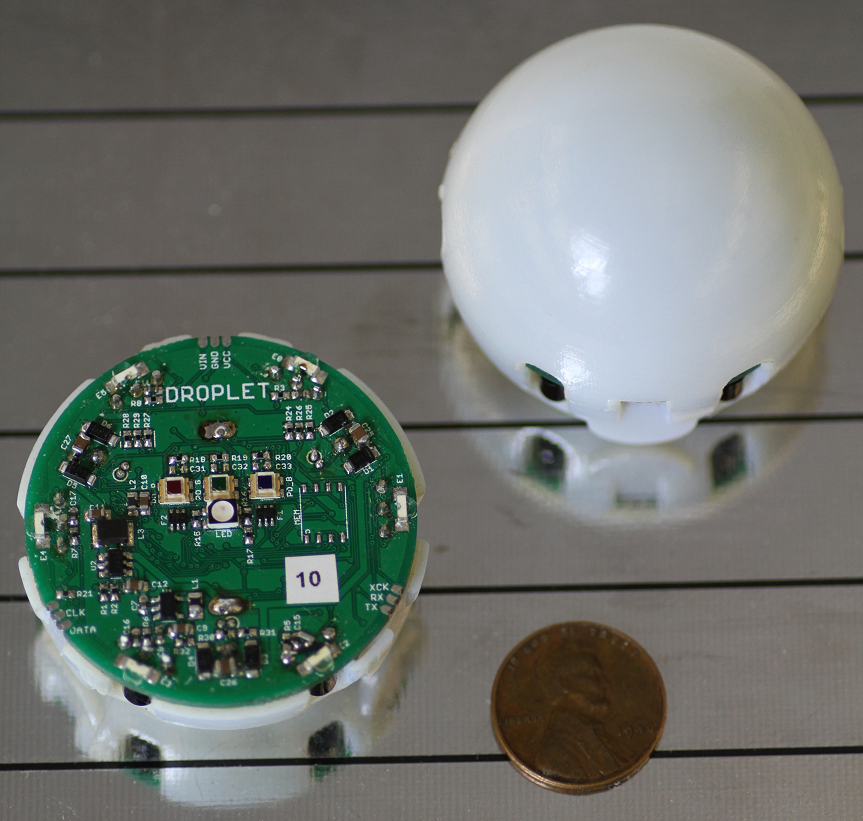
\includegraphics[width=\textwidth]{Images/droplets.png}
		\end{figure}
\end{columns}
		\begin{figure}
			\centering
			\makebox[\textwidth][c]{
			\subfile{singleDoFModelPresentation}
			}
		\end{figure}

\end{frame}
\begin{frame}
	\frametitle{The Method}
			\begin{itemize}
				\item Motors opposite legs.
				\item One motor on at a time gives `steps'.
					\note[item]<1->{Default 'on' time is 30ms. With calibration, this value is adjusted by ~10ms (on the high end) in either direction. 3ms is more typical.}
				\item Chain together a sequence of steps to walk.
			\end{itemize}
			\begin{figure}
				\centering
				\includegraphics[width=0.4\textwidth]{Images/step.png}
				\hspace{2em}
				\includegraphics[width=0.4\textwidth]{Images/walking.png}
			\end{figure}
			\begin{figure}
				\centering

			\end{figure}
\end{frame}
\end{document}